\label{quchempedia}

\par Ce travail s'inscrit dans le cadre du projet QuChemPedia\footnote{Quantum Chemistry Encyclopedia}. Il s'agit d'un projet de recherche mené à l'initiative de Thomas Cauchy et Benoit Da Mota, respectivement chercheurs à MOLTECH Anjou (laboratoire de recherche en chimie) et au LERIA (laboratoire de recherche en informatique). Ces deux laboratoires sont situés à la faculté des sciences d'Angers.\\

\begin{figure}
	\centering
	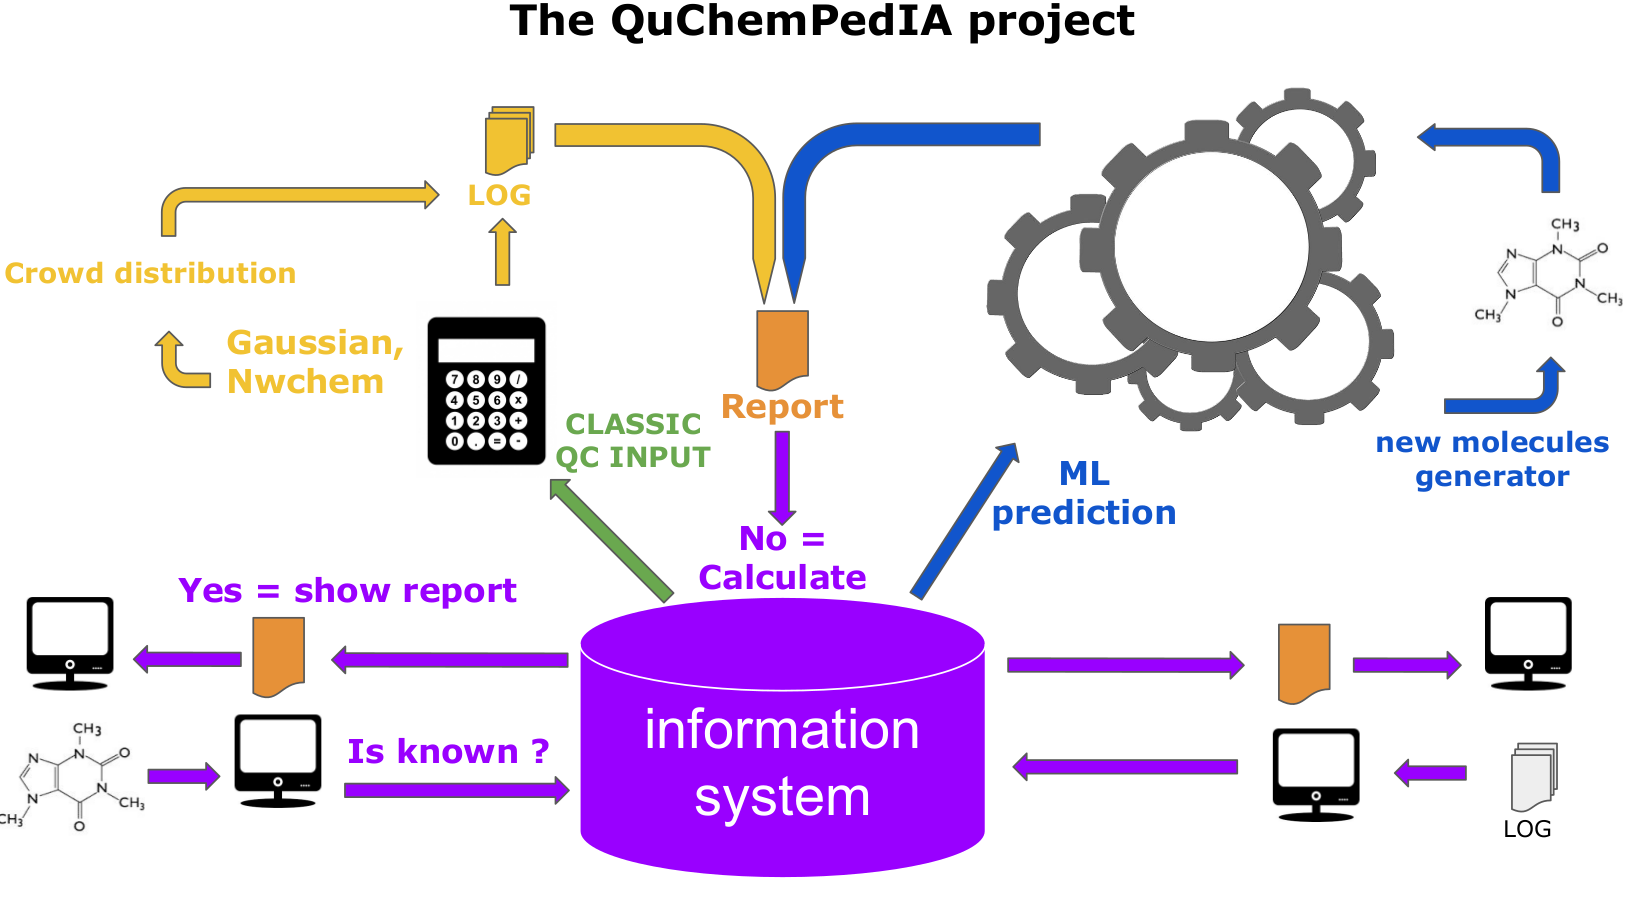
\includegraphics[scale=1]{images/part_proj.png}
	\caption{Synthèse des différents axes du projet QuChemPedia (T. Cauchy et B. Da Mota)}
	\label{figquchem}
\end{figure}

\par Il s'agit d'un projet ambitieux possédant de nombreux objectifs, représentés dans la figure \ref{figquchem}. L'objectif principal (en violet) est de mettre en place un système d'information de grande ampleur à destination des chimistes. Ce système d'information se présente sous forme d'un site web, leur permettant d'accéder à des calculs de chimie quantique.\par Ces calculs décrivent les différents états d'énergie des molécules, et représentent un second axe important (en jaune) du projet QuChemPedia. Ils sont en effet issus de divers programmes de chimie informatique (\ref{opti_geom}), dont les sorties diffèrent et sont peu structurées. Une partie importante du projet consiste alors à définir une représentation homogène des calculs provenant de ces différents programmes. Cette représentation, nommée rapport (en orange) est fournie aux utilisateurs effectuant une requête sur une molécule. Les chimistes possèdent également la possibilité de fournir les sorties des calculs qu'ils ont effectués, et d'obtenir les rapport associés.
\par Enfin, un objectif majeur du projet (en bleu) est de fournir une plus-value à ces rapports, issue de prédictions de modèles d'apprentissage automatique (\ref{apprentissage_auto}). Les calculs d'optimisation quantique sont en effet très coûteux (\ref{opti_geom}), le fait de les remplacer par des prédictions s'effectuant rapidement constituerait donc un apport très important.\\
Ce dernier axe du projet QuChemPedia est celui sur lequel j'ai travaillé cette année.


